\section{Twoverse System \& Library}
The software core of the August 23, 1966 project is a Java software system coined as "Twoverse," a parallel universe that exists only in the digital realm with some key points of connection to the real world. It can be considered an extension of the many-worlds interpretation - alongside our world, with its crumbling economies and warring nations, there exists a digital universe that is directed by you, the user. Just like here on Earth, many parameters are outside of your control. The interesting part is choosing what you can, timing as you may, and watching the results.

\begin{figure}[htp]\centering
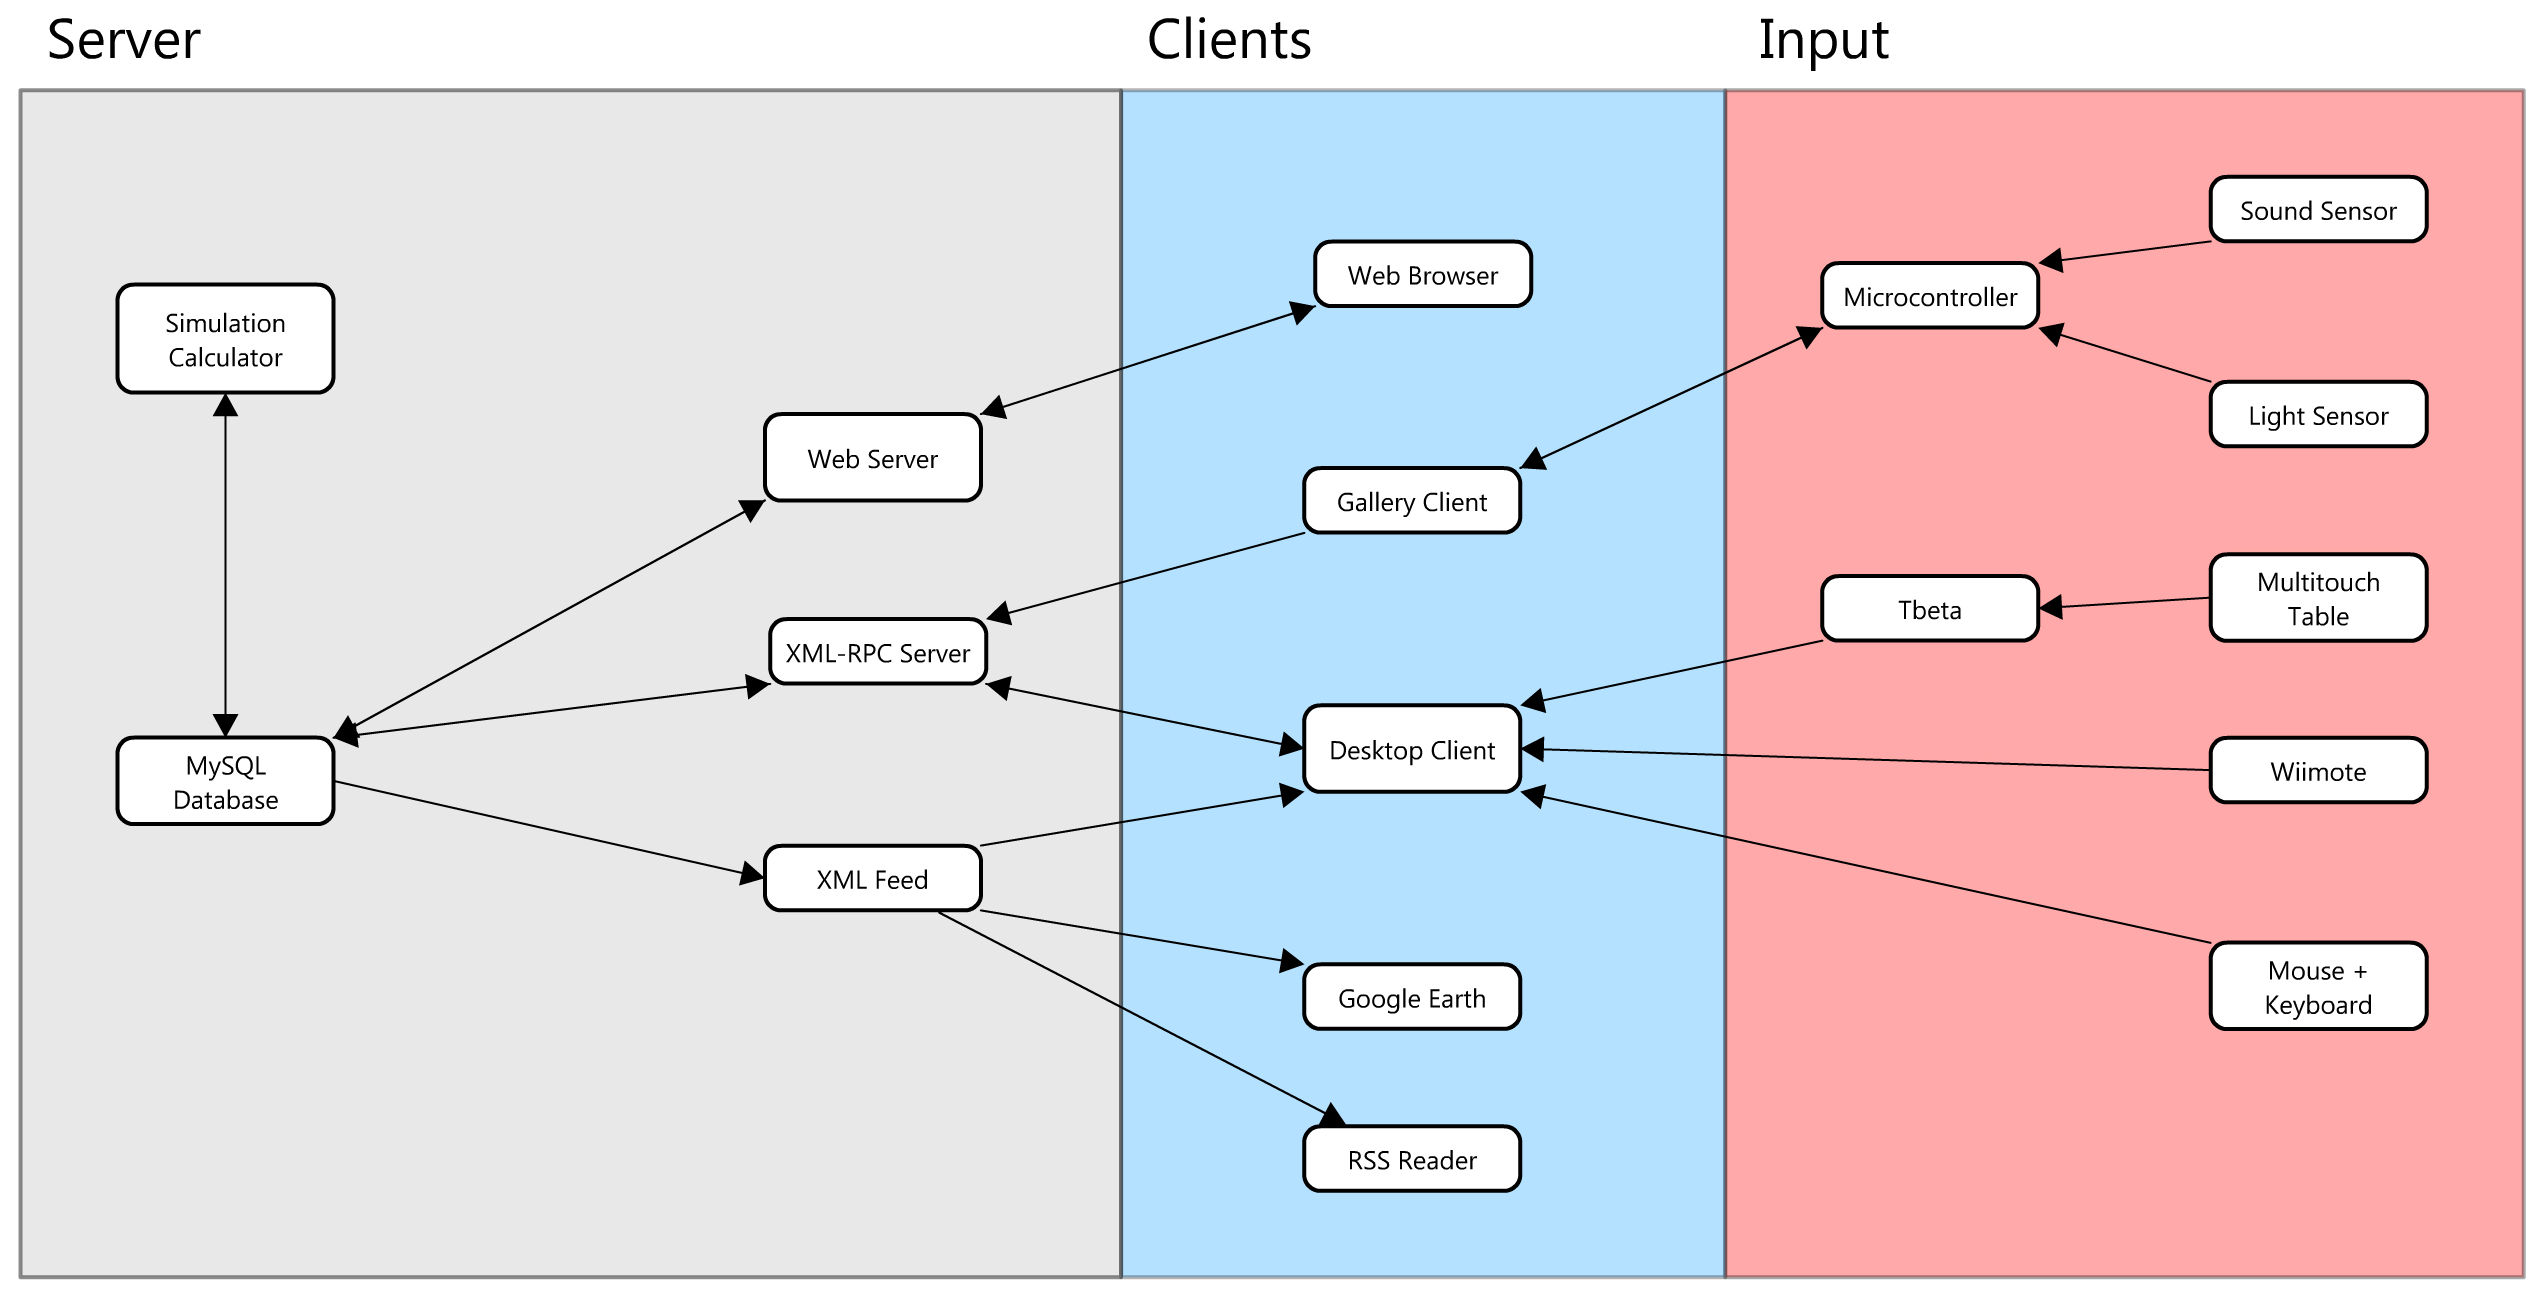
\includegraphics[width=.99\textwidth]{images/twoverse_arch.jpg}
  \caption{This is the Twoverse architecture!}\label{fig:twoversearch}
\end{figure}
\paragraph{System Design}
The broad concept of Twoverse includes mechanics and partial system specifications for a massively multiplayer online game. The scope was minimized due to time constraints and to better fit the gallery installation. However, even with a smaller scope, a complete vertical slice of the entire system was implemented and used. Downsized from a universe of many types of objects, the system currently supports a universe made of stars with a few properties, and constellations that connect them with meta-objects known as links. Scalability was stressed from the beginning of development, so extending the universe with new objects will require a minimal amount of work.

\paragraph{Server}
The system relies on a central server to provide the following:
\begin{itemize}
\item A persistant database of all objects in the universe and their current state, using MySQL
\item User account management, as well as authenticated session negotiation
\item A public API for interacting with the universe, via Apache XML-RPC \cite{XMLRPC}
\item Client pull style updates for minimizing bandwidth requirements, via an XML feed
\item A web-browser based frontend to view the status of objects in the universe, via PHP
\end{itemize}

\paragraph{Client}
Using the public API, many types of clients are possible. This includes graphical, text-based, mobile, e-mail, etc. The clients implemented for the gallery installation are graphical clients written using the Processing development environment and include the following features:
\begin{itemize}
\item Users can scroll and zoom around a graphical universe of glowing stars
\item Users can click on an individual star to view a close-up view and additional details about its creation and properties
\item Users can create a new star in the universe, and watch a 3D visualization of their star's formation
\item Users can draw constellations that connect the stars in the universe, and leave them for other users to see
\item Users can visit the gallery website to view a table of all of the stars in the universe, their properties and current status (see figure \ref{fig:starchart})
\end{itemize}
The graphical client uses the XML-RPC API as defined by the server, and updates its local cache of the universe via the server's XML feed.
\begin{figure}[htp]\centering
  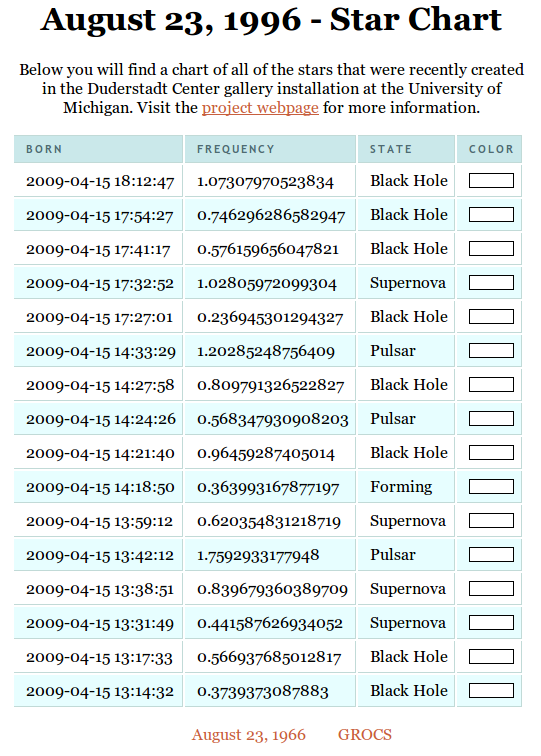
\includegraphics[width=.4\textwidth]{images/starchart.png}
  \caption{This is the star chart!}\label{fig:starchart}
\end{figure}
\paragraph{Library}
The client and server for Twoverse share many common functions, and were designed to inherit their source from the same tree of code. They both stem from a Twoverse Java library, which includes many utility classes, shared functionality and the server executable. The Twoverse library provides these features and many others:
\begin{itemize}
\item Database wrapper class for a persistant universe - could be used to run SQL database client-side
\item XML-RPC servlet for serving XML-RPC requests
\item Thread-safe universal object manager for maintaining the state of the universe
\item User session manager
\item Small unit test suite for core classes
\item Processing camera wrapper class for simplifying the elusive camera() function
\item Flexible 2D/3D point coordinate class
\end{itemize}
The source code as well as an extensive HTML reference is included in the software package at \texttt{/august/src/Twoverse/doc} \cite{PACK}.
\paragraph{}
See the project wiki \cite{WIKI} for more information on the motive for Twoverse and possible future plans.
